\documentclass[a4paper, 12pt]{article}

\usepackage{cmap}
\usepackage{mathtext} 
\usepackage[T2A]{fontenc}
\usepackage[utf8]{inputenc}
\usepackage[english,russian]{babel}	

\usepackage{amsfonts,amssymb,amsthm,mathtools}
\usepackage{amsmath}
\usepackage{icomma} 

\usepackage{graphicx} 
\graphicspath{{Picturies/}}
\usepackage{wrapfig}

\usepackage{array,tabularx,tabulary,booktabs}
\usepackage{longtable}
\usepackage{multirow}

\usepackage{caption}
\captionsetup{labelsep=period}

\renewcommand{\phi}{\varphi}
\newcommand{\eps}{\varepsilon}
\renewcommand{\AA}{\ensuremath{\mathring{A}}}
\newcommand{\parag}[1]{\paragraph*{#1:}}

\newcounter{Points}
\setcounter{Points}{1}
\newcommand{\point}{\arabic{Points}. \addtocounter{Points}{1}}

\author{Вязовцев Андрей, Б01-005}
\date{11.02.22}
\title{Лабораторная работа 4.2.3. }

\begin {document}

\maketitle

\parag {Цель работы} знакомство с устройством и принципом действия интерферометра Релея и с его применением для измерения показателей преломления газов.

\parag {В работе используются} технический интерферометр ИТР-1, светофильтр, баллон с углекислым газом, сильфон, манометр, краны.

% \parag {Теоретическая справка} ~\\ % ToDo

\parag {Экспериментальная установка} ~

Интерферометр Релея --- прибор для измерения разности показателей преломления --- основан на явлении дифракции света на двух параллельных щелях.

\begin{figure}[!h]
    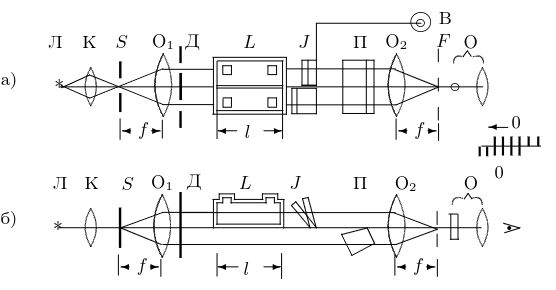
\includegraphics[scale = 1]{Workplace}
    \centering
    \caption{Устройство интерферометра Релея: а) вид сверху; б)вид сбоку}
\end{figure}

\parag {Ход работы} ~\\

\point Осмотрим установку и подготовим к работе: выравняем давления в камерах, продуем камеру с углекислым газом. Подождём, пока выравняются температуры. Совместим полосы (сначала боковые, потом центральные).

\point Возьмём красный светофильтр (диапазон волн $6200-7200~\AA$) и откалибруем с помощью него компенсатор в единицах $\lambda$. Для этого будем последовательно совмещать подвижные полосы с нулевой неподвижной и зафиксируем показания микрометра. Результаты см. в таблице \ref{kalib}.

\begin{table}[!h]
    \centering
    \begin{tabular}{|c|c|c|c|c|c|c|c|c|}
        \hline
        m (№ линии) & 5 & 4 & 3 & 2 & 1 & 0 & 1 & 2 \\ \hline
        z, мм & 0.80 & 1.40 & 1.72 & 2.05 & 2.41 & 2.73 & 3.03 & 3.37 
        \\ \hline \multicolumn{9}{c}{ } \\ \hline
        m (№ линии) & 3 & 4 & 5 & 6 & 7 & 8 & 9 & 10 \\ \hline
        z, мм & 3.69 & 4.03 & 4.36 & 4.66 & 4.98 & 5.30 & 5.64 & 5.94
        \\ \hline
    \end{tabular}
    \caption {Показания микрометра}
    \label{kalib}
\end{table}

\point Запишем характеристики установки:

Диапазон светофильтра: $6200-7200~\AA$

Длина волны светофильтра: $\lambda = 6700~\AA$

Длина кюветы: $l = 10~см$

\point Будем изменять давление в одной из камер, компенсатором совмещать нулевые полосы и записывать показания микрометра. Результаты см. в таблице \ref{press}. Стоит отметить, что здесь, видимо, у  были перепутанны выходы на атмосферу и камеру. Далее все значения давления будут умножены на $-1$.

\begin{table}[!h]
    \centering
    \begin{tabular}{|c|c|c|c|c|c|c|c|c|c|c|c|}
        \hline
        $\Delta P$, мм.в. ст. & -1000 & -900 & -800 & -700 & -600 & -500 & -400 & -300 & -200 & -100 & 0 \\ \hline
        $z$, мм & 4.07 & 3.92 & 3.74 & 3.65 & 3.54 & 3.45 & 3.23 & 3.14 & 3.00 & 2.86 & 2.76 \\ \hline
        \multicolumn{12}{c}{ } \\ \hline
        $\Delta P$, мм.в. ст. & 0 & 100 & 200 & 300 & 400 & 500 & 600 & 700 & 800 & 900 & 1000 \\ \hline
        $z$, мм & 2.76 & 2.55 & 2.46 & 2.36 & 2.19 & 1.99 & 1.86 & 1.72 & 1.53 & 1.29 & 1.03 \\ \hline
    \end{tabular}
    \caption {Зависимость смещения от давления}
    \label{press}
\end{table}

\point Теперь одну камеру наполним углекислым газом, а другую --- воздухом (обе при атмосферном давлении). Т.к. камеры могут <<подтекать>>, положение равновесия будет смещаться со временем. Измерим зависимость показаний микрометра от времени. Результаты приведены в таблице \ref{CO2_1}.

\begin{table}[!h]
    \centering
    \begin{tabular}{|c|c|c|c|c|c|c|c|c|c|c|c|}
        \hline
        $t$, мин & 0 & 1 & 2 & 3 & 4 & 5 & 6 & 7 & 8 & 9 & 10 \\ \hline
        $z$, мм & 9.90 & 8.86 & 7.89 & 7.50 & 6.58 & 6.00 & 5.42 & 5.07 & 4.81 & 4.45 & 4.30 \\ \hline
    \end{tabular}
    \caption {Зависимость смещения от времени}
    \label{CO2_1}
\end{table}

Повторим измерения (см. таблицу \ref{CO2_2}).

\begin{table}[!h]
    \centering
    \begin{tabular}{|c|c|c|c|c|c|c|}
        \hline
        $t$, мин & 0 & 1 & 2 & 3 & 4 & 5\\ \hline
        $z$, мм & 9.99 & 8.73 & 7.78 & 7.37 & 6.82 & 6.25 \\ \hline
    \end{tabular}
    \caption {Зависимость смещения от времени}
    \label{CO2_2}
\end{table}

\point Определим температуру и давление в лаборатории: $T = 22.2^\circ C$, $P = 100.2$ кПа.

\point На месте оценим интервал $\delta n$, доступный для измерений. Можно считать, что коэфициент преломления не значительно отличается от табличного ($n = 1.00027$). Точность прибора равна $0.01$ мм., а диапазон его работы составляет $30$ мм. Подставляя эти значения вместо $\Delta$ в формуле:

\[
    n = n_{возд} + \frac{\Delta}{l}
\]

получим: $\delta n = [1.00037; 1.03]$

\parag {Обработка результатов} ~\\

\point Построим график $z (m)$ по таблице \ref{kalib}. См. рис. \ref{img:kalib}.

\begin{figure}[!h]
    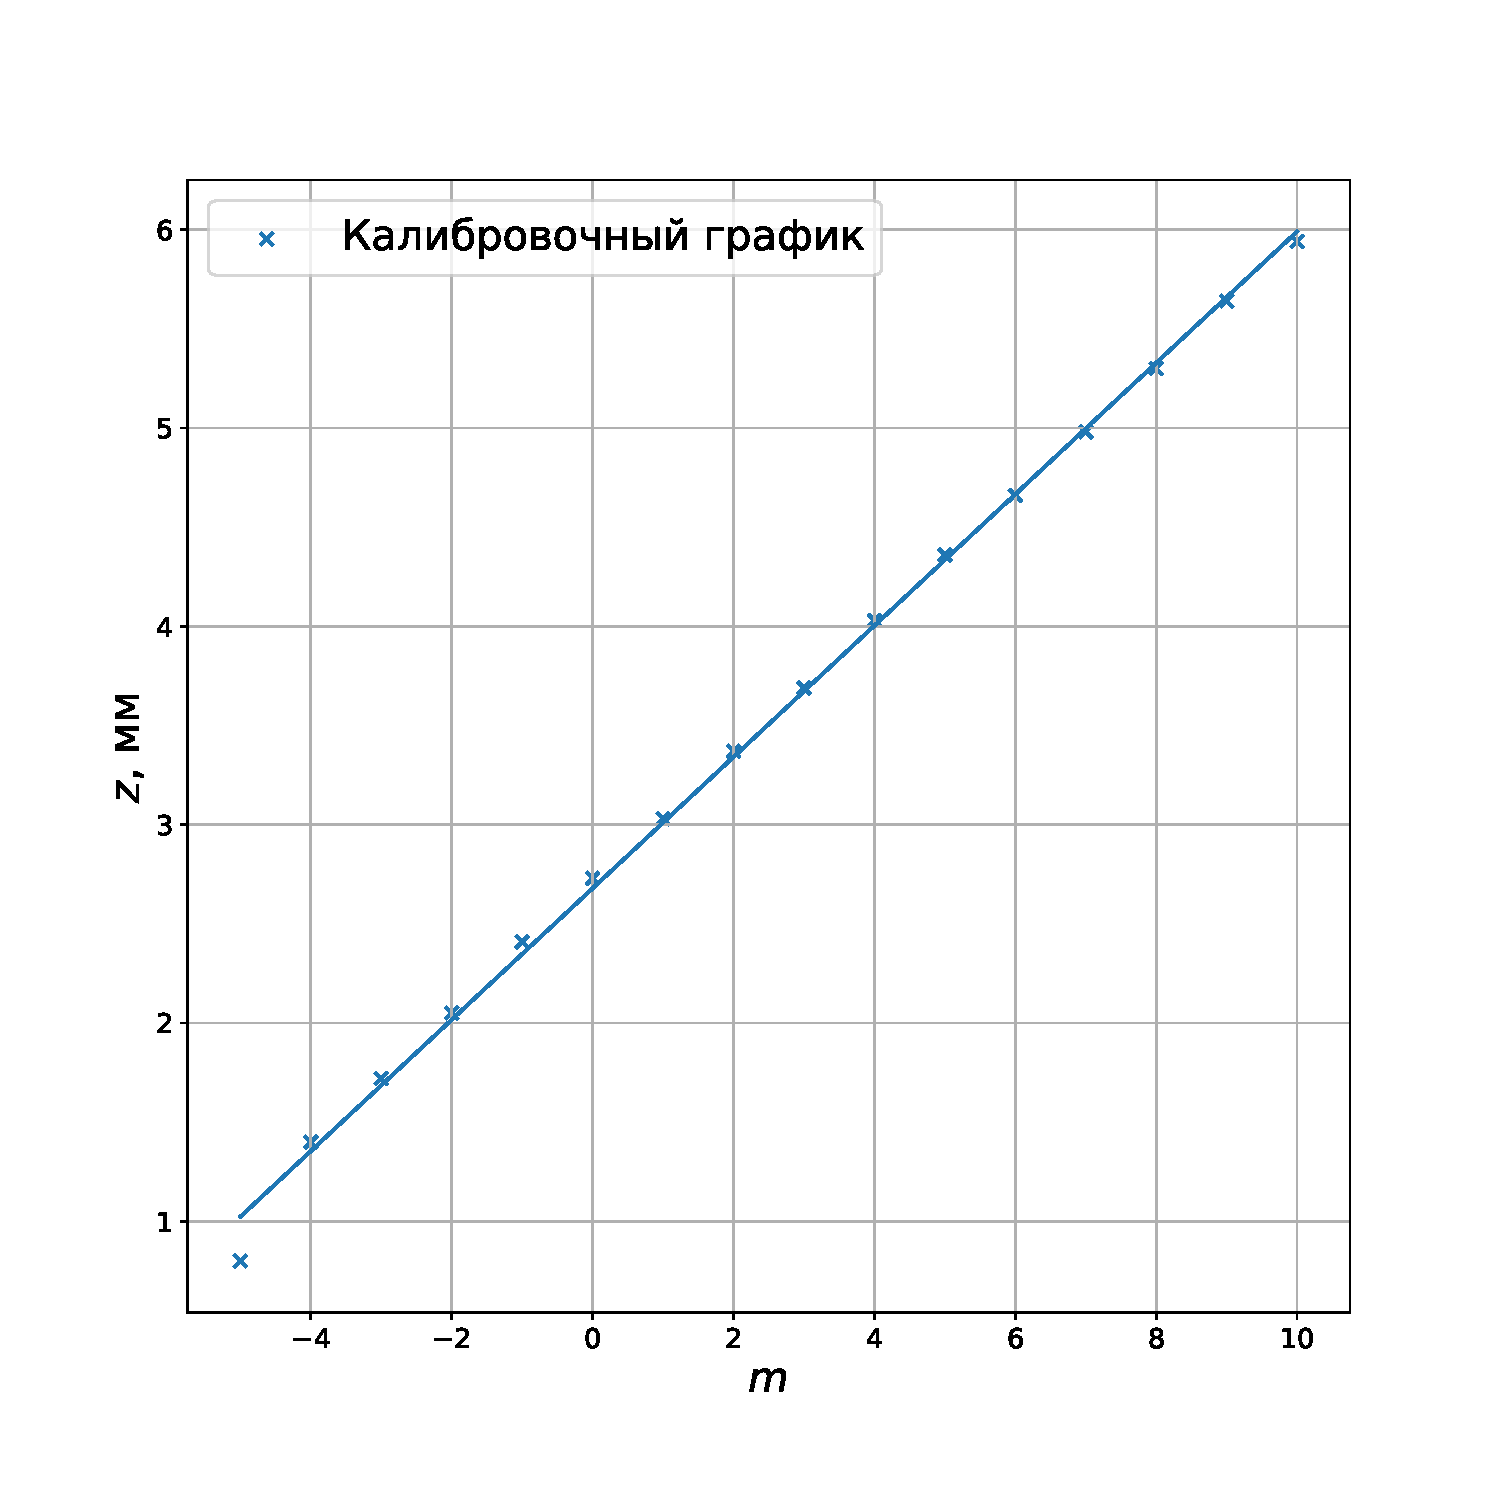
\includegraphics[scale = 0.5]{kalib}
    \centering
    \caption{Калибровочный график}
    \label{img:kalib}
\end{figure}

\point Теперь с помощью предыдущего графика и таблицы \ref{press} построим график $\Delta n (\Delta P)$ (см. рис. \ref{img:press}). Для этого воспользуемся формулой:

\[
    \Delta n = m \frac{\lambda}{l}
\]

Далее, после построения, найдём среднюю поляризуемость молекулы воздуха:

\[
    \alpha = \frac{\Delta n}{\Delta P} \cdot \frac{kT}{2 \pi}
\]

После посчитаем показатель преломления воздуха в условиях опыта:

\[
    n = 1 + 2 \pi \alpha \frac{P}{kT}
\]

Теперь получим показатель преломления воздуха по формуле, сравним его с табличным:

\[
    \frac{n_0-1}{n-1} = \frac{T}{T_0} \cdot \frac{P_0}{P}
\]

\begin{figure}[!h]
    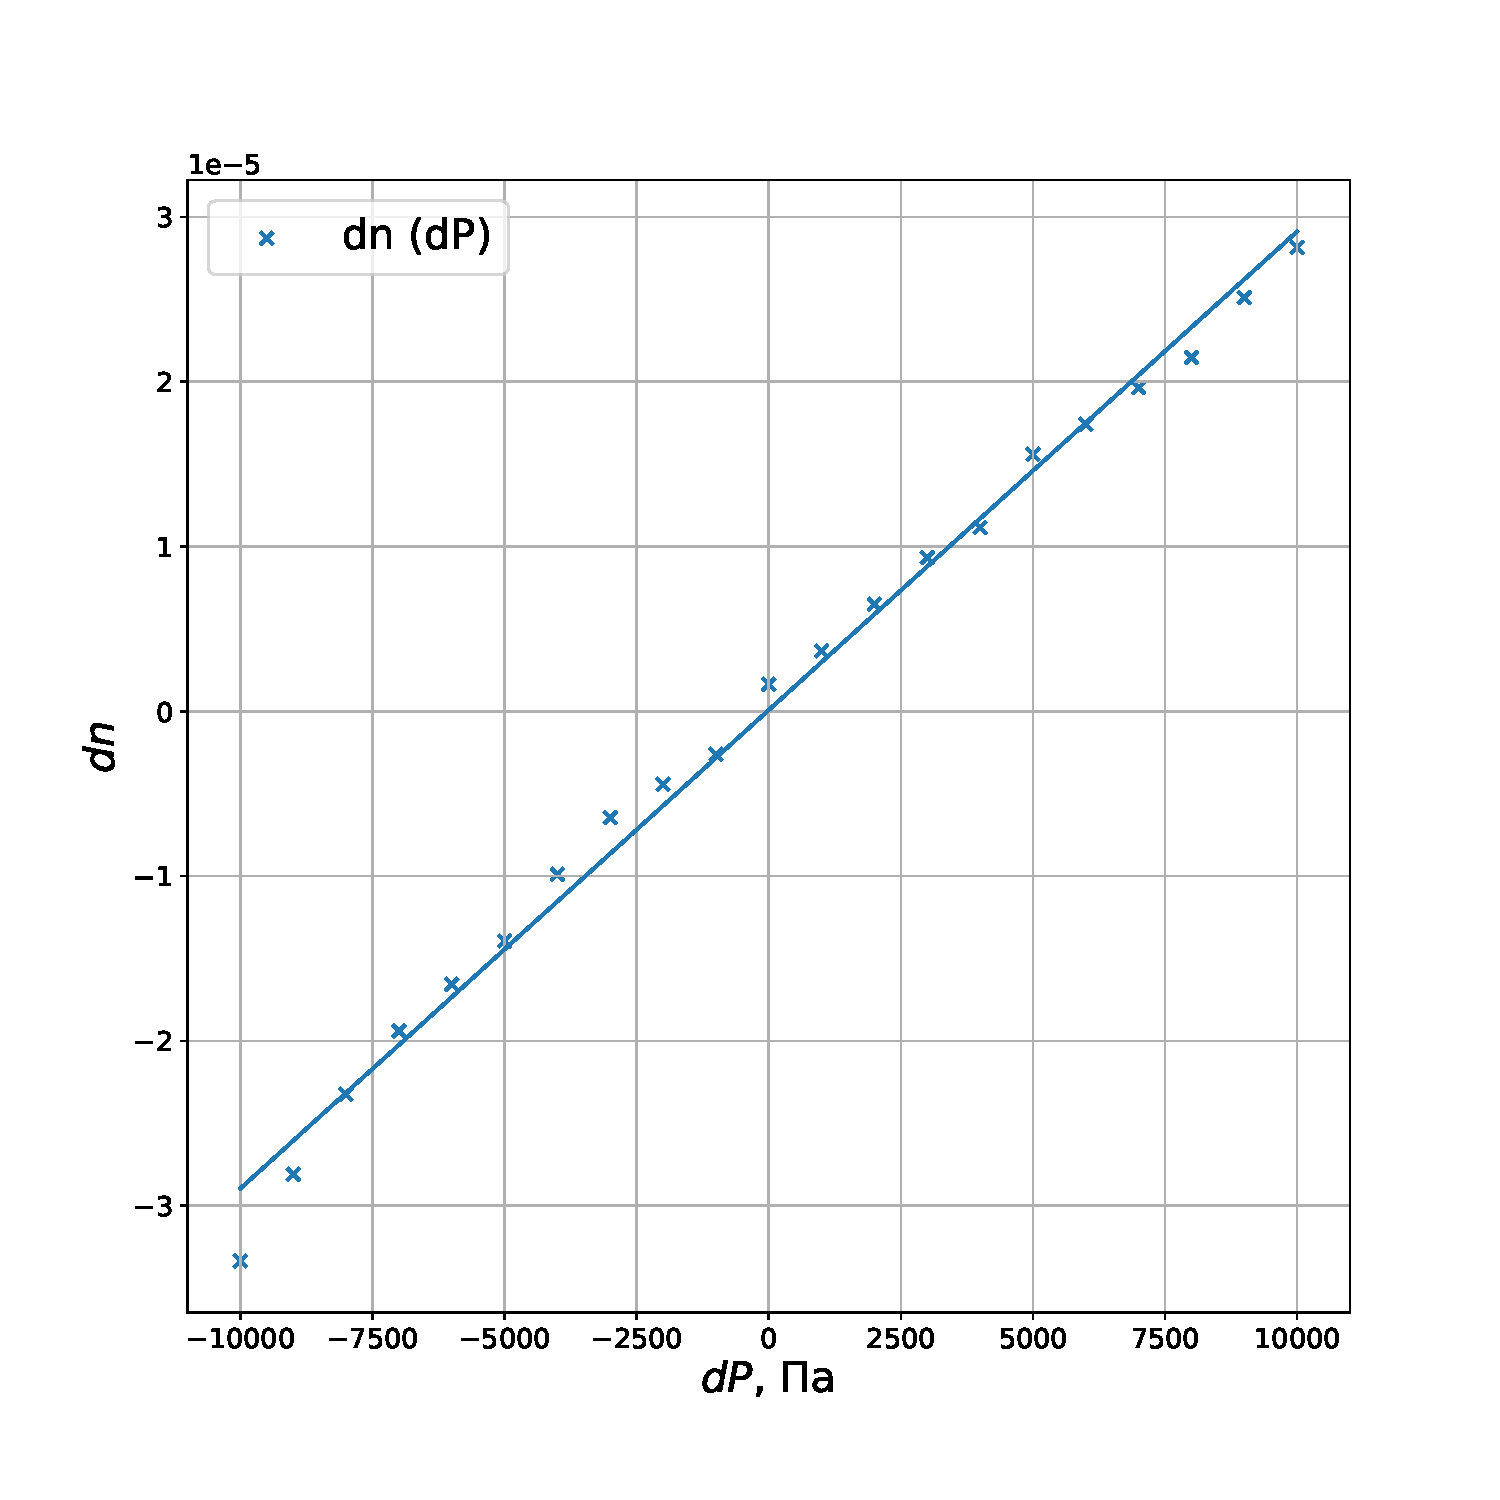
\includegraphics[scale = 0.5]{press}
    \centering
    \caption{$\Delta n (\Delta P)$}
    \label{img:press}
\end{figure}

Коэффициент наклона этой прямой: $\frac{\Delta n}{\Delta P} = (2.90 \pm 0.5) \cdot 10^{-9}$

Следовательно, получаем:

\begin{align*}
    \alpha &= (1.7 \pm 0.2) \cdot 10^{-30} ~м^3 \\
    n_{возд} &= 1.00026 \pm 0.00003 \\
    n_{возд-норм} &= 1.00033 \pm 0.00003 
\end{align*}

Что довольно близко к табличным значениям: $n_{возд-норм} = 1.00027$

\point Теперь можно вычислить показатель преломления углекислого газа по следующей формуле:

\[
    n = n_{возд} + \frac{\Delta}{l}
\]

После можно, по аналогии с предыдущем пунктом, найти показатель преломления при нормальных условиях.

\begin{align*}
    n_{CO_2} &= 1.00040 \pm 0.00004 \\
    n_{CO_2-норм} &= 1.00051 \pm 0.00005 
\end{align*}

Табличный же показатель преломления $n_{CO_2-норм} = 1.00045$, что согласуется с экспериментом.

\end {document}
